\documentclass[12pt]{article}

\usepackage{sbc-template}

\usepackage{graphicx,url}

\usepackage[brazil]{babel}
\usepackage[utf8]{inputenc}
\sloppy

\title{Predição de Churn e Segmentação Encadeada de Clientes em Risco no Setor de Telecomunicações}

\author{Matheus Eduardo Laurindo do Rego\inst{1}}


\address{Especialização em Ciência de Dados\\
Universidade Tecnológica Federal do Paraná (UTFPR)
  \email{matheusrego@alunos.utfpr.edu.br}
}

\begin{document}

\maketitle

\begin{abstract}
  This work presents a two-stage churn pipeline on the public IBM Telco Customer
  Churn dataset (7,043 customers). First, Random Forest, XGBoost and LightGBM are
  tuned with Optuna over a composite objective balancing F-measure and accuracy,
  with a calibrated decision threshold. XGBoost was selected, reaching AUC-ROC of
  0.847, accuracy of 80.6\% and precision of 66.4\% on the hold-out set, and SHAP
  values show that engineered features dominate the prediction. Second, only the
  customers flagged as at risk (1,556 or 22.1\% of the base) are segmented with
  K-Means (K = 3), yielding three actionable profiles that expose R\$ 123.4k of
  monthly revenue at risk, 59.0\% of it in a single segment, which supports a
  differentiated retention playbook.
\end{abstract}

\begin{resumo}
  Este trabalho apresenta um \textit{pipeline} de churn em duas etapas sobre a
  base pública IBM Telco Customer Churn (7.043 clientes). Na primeira, Random
  Forest, XGBoost e LightGBM são otimizados com Optuna sobre um objetivo composto
  que equilibra F-medida e acurácia, com limiar de decisão calibrado. O XGBoost
  foi selecionado, alcançando AUC-ROC de 0,847, acurácia de 80,6\% e precisão de
  66,4\% no teste, e a análise SHAP mostra que as variáveis derivadas dominam a
  predição. Na segunda, apenas os clientes sinalizados como em risco (1.556, ou
  22,1\% da base) são segmentados com K-Means (K = 3), gerando três perfis
  acionáveis que expõem R\$ 123,4 mil de receita mensal em risco, com 59,0\% em
  um único segmento, o que fundamenta um plano de retenção diferenciado.
\end{resumo}


\section{Introdução}

No setor de telecomunicações, o custo de aquisição de um novo cliente é
substancialmente maior que o custo de retenção de um cliente existente, o que
torna a gestão do cancelamento de serviços --- comumente chamado de
\textit{churn} --- uma das principais alavancas de resultado das operadoras
\cite{hadden2007, verbeke2012}. A digitalização dos canais de atendimento e a
oferta de planos sem fidelidade tornaram a troca de operadora uma decisão de
baixo atrito para o consumidor, ampliando a exposição da receita recorrente.

A resposta usual da área de Ciência de Dados a esse problema é o modelo de
classificação binária que estima a probabilidade de cancelamento de cada
cliente. Esse tipo de modelo, isoladamente, resolve apenas metade do problema:
ele indica \textit{quem} está em risco, mas não indica \textit{o que fazer} com
cada cliente identificado. Na prática comercial, uma lista de milhares de
clientes em risco sem qualquer qualificação de perfil tende a receber um
tratamento único, o que desperdiça orçamento de retenção em clientes de baixo
valor e oferece resposta genérica a clientes de alto valor.

Este trabalho aborda essa lacuna por meio de um \textit{pipeline} encadeado em
duas etapas. A primeira etapa é um classificador de churn com limiar de decisão
calibrado, que sinaliza um subconjunto da base como em risco. A segunda etapa
aplica agrupamento não supervisionado \textbf{exclusivamente sobre esse
subconjunto}, de modo que os segmentos resultantes não descrevem a base inteira,
mas sim a população que o modelo considera prioritária para ação. Cada segmento
é então traduzido em métricas de negócio (volume de clientes, receita mensal
exposta) e em uma recomendação de retenção específica.

O estudo utiliza a base pública IBM Telco Customer Churn \cite{ibm2018}, com
7.043 clientes e 21 atributos. O contexto de aplicação é o de uma operadora
brasileira de banda larga: identificar assinantes com propensão a cancelar e
qualificá-los por perfil comportamental para direcionar ações comerciais
diferenciadas. Como a base real da operadora não pode ser divulgada, a base
pública foi adotada como \textit{proxy}, mantendo a estrutura de atributos
típica do setor (tipo de contrato, forma de pagamento, tipo de acesso à
internet, serviços agregados e faturamento).

As contribuições do trabalho são: (i) um \textit{pipeline} reprodutível e
modular de seis etapas, da extração à recomendação comercial; (ii) uma
estratégia de otimização orientada a um objetivo composto entre F-medida e
acurácia, com calibração explícita do limiar de decisão, em vez do limiar
padrão de 0,5; (iii) a segmentação encadeada dos clientes sinalizados, com
tradução dos segmentos em receita exposta e plano de ação; (iv) a análise de
interpretabilidade com valores SHAP, que verifica se os fatores usados pelo
modelo são coerentes com os achados da análise exploratória; e (v) uma discussão
crítica das limitações observadas, incluindo o teto empírico de desempenho da
base utilizada.

O texto está organizado da seguinte forma: a Seção \ref{sec:2} apresenta os
trabalhos relacionados. A Seção \ref{sec:3} descreve a metodologia utilizada.
Os resultados experimentais estão na Seção \ref{sec:4}. Por fim, a
Seção \ref{sec:5} apresenta a conclusão e propostas de trabalhos futuros.

\section{Trabalhos Relacionados}
\label{sec:2}

A predição de churn em telecomunicações é um problema consolidado na
literatura. \cite{hadden2007} revisaram o estado da arte da gestão assistida
por computador do churn e apontaram que, à época, a maior parte dos trabalhos
concentrava-se na acurácia preditiva, com pouca atenção à conexão entre a
predição e a ação de retenção. Essa crítica permanece pertinente e motiva
diretamente o desenho adotado neste trabalho.

\cite{verbeke2012} conduziram um dos \textit{benchmarks} mais amplos da área,
avaliando diversos classificadores sobre onze bases reais de operadoras. Duas
conclusões daquele estudo orientaram decisões metodológicas aqui: um número
reduzido de variáveis costuma ser suficiente para prever churn com boa
qualidade, e a reamostragem por sobreamostragem geralmente não produz ganho
significativo de desempenho. Os autores também propuseram uma medida de
desempenho orientada a lucro, argumentando que métricas puramente estatísticas
levam à seleção subótima de modelos --- ideia próxima da adotada neste trabalho,
onde a escolha do limiar de decisão privilegia precisão em razão do custo
operacional do contato comercial.

\cite{ahmad2019} desenvolveram um modelo de churn sobre dados reais de uma
operadora, comparando árvore de decisão, Random Forest, GBM e XGBoost em
plataforma de \textit{big data}, com AUC de 93,3\% após a incorporação de
atributos de análise de redes sociais. O trabalho é uma referência relevante de
desempenho, mas o valor elevado de AUC é obtido com atributos de rede e de
consumo temporal indisponíveis na base pública utilizada aqui, o que ajuda a
contextualizar a diferença de patamar observada nos resultados desta seção
experimental.

Especificamente sobre o encadeamento entre classificação e agrupamento,
\cite{bose2009} investigaram modelos híbridos de dois estágios, combinando
técnicas de agrupamento não supervisionado (K-Means, K-Medoid, mapas
auto-organizáveis, \textit{fuzzy c-means} e BIRCH) com árvores de decisão com
\textit{boosting}, e observaram ganho de \textit{top decile lift} em relação ao
cenário sem agrupamento. Naquele estudo, porém, o agrupamento antecede a
classificação e serve como insumo preditivo. \cite{ullah2019} propuseram a
ordem inversa, mais próxima da adotada neste trabalho: primeiro classificam os
clientes com Random Forest (88,63\% de instâncias corretamente classificadas) e
depois agrupam os clientes identificados como churn para gerar ofertas de
retenção por grupo, além de extrair os fatores associados ao cancelamento.

O presente trabalho se posiciona nessa mesma linha de dois estágios com
classificação seguida de agrupamento, e se diferencia em três pontos. Primeiro,
o agrupamento opera sobre a saída operacional do modelo --- os clientes
sinalizados pelo limiar calibrado, que incluem falsos positivos --- e não sobre
o rótulo verdadeiro de churn, refletindo a condição real de uso em que o rótulo
é desconhecido no momento da ação. Segundo, a otimização de hiperparâmetros é
conduzida por busca bayesiana \cite{akiba2019} sobre um objetivo composto que
equilibra F-medida e acurácia, com o limiar de decisão otimizado dentro de cada
avaliação. Terceiro, cada segmento é quantificado em receita mensal exposta e
associado a um plano de ação com indicador de acompanhamento, fechando o ciclo
entre modelo e decisão comercial apontado por \cite{hadden2007}.

\section{Metodologia}
\label{sec:3}

O trabalho foi implementado em Python 3.12 e organizado em seis notebooks
sequenciais, cada um autônomo e responsável por uma etapa do
\textit{pipeline}, com persistência dos artefatos intermediários em disco no
formato Parquet. A Tabela \ref{tab:pipeline} resume as etapas. As bibliotecas
principais são \textit{pandas} e \textit{numpy} para manipulação de dados,
\textit{scikit-learn} \cite{pedregosa2011} para pré-processamento, agrupamento e
métricas, \textit{xgboost} \cite{chen2016} e \textit{lightgbm} \cite{ke2017}
para os modelos de \textit{gradient boosting}, \textit{optuna}
\cite{akiba2019} para otimização de hiperparâmetros e \textit{joblib} para
serialização dos modelos.

\begin{table}[ht]
\centering
\caption{Etapas do \textit{pipeline} e artefatos gerados.}
\label{tab:pipeline}
\small
\begin{tabular}{|c|l|l|}
\hline
\textbf{Etapa} & \textbf{Descrição} & \textbf{Artefato de saída} \\
\hline
NB01 & Extração e consolidação      & \texttt{base\_consolidada.parquet} \\ \hline
NB02 & Análise exploratória         & --- (diagnóstico) \\ \hline
NB03 & Engenharia de \textit{features} e divisão & \texttt{treino/teste\_modelagem.parquet} \\ \hline
NB04 & Classificação e SHAP         & \texttt{modelo\_churn.pkl} \\
     &                              & \texttt{clientes\_em\_risco.parquet} \\ \hline
NB05 & Segmentação dos sinalizados  & \texttt{clientes\_segmentados.parquet} \\ \hline
NB06 & Relatório de impacto         & \texttt{relatorio\_final.parquet} \\
\hline
\end{tabular}
\end{table}

\subsection{Base de dados e consolidação}
\label{sub:base}

A base IBM Telco Customer Churn \cite{ibm2018} contém 7.043 registros e 21
colunas, com um cliente por linha e nenhuma dimensão temporal explícita. Os
atributos cobrem dados demográficos (gênero, idade sênior, presença de parceiro
e de dependentes), contratuais (tipo de contrato, forma de pagamento, fatura
digital), de serviços (telefonia, tipo de internet, segurança
\textit{online}, \textit{backup}, proteção de dispositivo, suporte técnico e
\textit{streaming}) e financeiros (tempo de relacionamento em meses, fatura
mensal e fatura acumulada). A variável alvo é binária e indica se o cliente
cancelou o serviço.

Na consolidação, três tratamentos foram aplicados. A coluna de fatura acumulada
era do tipo textual e foi convertida para numérico; a conversão revelou 11
registros vazios, todos correspondentes a clientes com tempo de relacionamento
igual a zero, ou seja, assinantes recém-ativados que ainda não geraram fatura,
tratados com preenchimento por zero. A variável alvo foi convertida para
representação binária. Por fim, as categorias \textit{No internet service} e
\textit{No phone service}, presentes em sete colunas de serviços, foram
unificadas em \textit{No}, uma vez que codificam a ausência do serviço de forma
redundante com as colunas de serviço base. Ao final, verificou-se a unicidade do
identificador de cliente e a ausência de valores nulos.

\subsection{Análise exploratória}

A análise exploratória foi conduzida sob três lentes: perfil de churn (recortes
demográficos e contratuais), comportamento financeiro (fatura mensal, fatura
acumulada e tempo de relacionamento) e uso de serviços agregados. Para as
variáveis numéricas, a comparação entre os grupos que cancelaram e que
permaneceram foi avaliada com o teste não paramétrico de Mann-Whitney, dada a
assimetria das distribuições, e a associação com a variável alvo foi medida pela
correlação de Spearman, adequada a relações monotônicas não necessariamente
lineares. Os achados desta etapa orientaram diretamente a engenharia de
atributos descrita a seguir.

\subsection{Engenharia de \textit{features} e preparação}
\label{sub:features}

A partir das 21 colunas originais foram derivados atributos em quatro grupos.
O primeiro é de tempo de relacionamento, com faixas discretizadas (0--12,
13--24, 25--48 e 49--72 meses) e um indicador de cliente novo (até 12 meses).
O segundo é financeiro, com a fatura média por mês de permanência e o desvio da
fatura mensal em relação à média do respectivo tipo de contrato, que mede se o
cliente paga acima ou abaixo dos seus pares contratuais. O terceiro é de
serviços, com a contagem de serviços agregados, a contagem de serviços de
proteção e indicadores de ausência total de serviços ou de proteção. O quarto
grupo é de risco e interação, incluindo um escore de risco obtido pela soma de
indicadores associados a maior propensão de cancelamento (contrato mensal, fibra
óptica, pagamento por boleto eletrônico, cliente sênior, ausência de suporte
técnico e ausência de segurança \textit{online}) e termos de interação entre
contrato mensal e perfil do cliente, sugeridos pela exploração.

As variáveis categóricas binárias foram codificadas com \textit{LabelEncoder} e
as multiclasse (tipo de internet, tipo de contrato, forma de pagamento e faixa
de tempo de relacionamento) com codificação \textit{one-hot}. Sete indicadores
que se tornaram redundantes após a codificação \textit{one-hot} foram removidos,
resultando em 47 atributos de modelagem. Cópias não normalizadas de fatura
mensal, fatura acumulada e tempo de relacionamento foram preservadas para
interpretação posterior das métricas de negócio.

A divisão treino/teste foi estratificada pela variável alvo, na proporção
80/20, resultando em 5.634 amostras de treino e 1.409 de teste, ambas com 26,5\%
de churn. A padronização por média e desvio padrão foi aplicada às dez colunas
numéricas contínuas, com o escalonador ajustado \textbf{apenas} nos dados de
treino e posteriormente aplicado ao teste, evitando vazamento de informação.

\subsection{Modelagem de churn}
\label{sub:modelagem}

Três algoritmos de conjunto foram comparados: Random Forest
\cite{breiman2001}, XGBoost \cite{chen2016} e LightGBM \cite{ke2017}. O
desbalanceamento de classes (razão de 2,77 entre não churn e churn no treino)
foi tratado por ponderação de classes --- \textit{class\_weight} balanceado no
Random Forest e \textit{scale\_pos\_weight} nos modelos de \textit{boosting},
com o próprio fator de ponderação incluído no espaço de busca --- e não por
sobreamostragem sintética \cite{chawla2002}, decisão alinhada ao achado de
\cite{verbeke2012} de que a sobreamostragem raramente traz ganho relevante
neste domínio.

A otimização de hiperparâmetros usou o \textit{framework} Optuna
\cite{akiba2019} com 40 tentativas por algoritmo. A função objetivo foi
definida como um escore composto entre F-medida e acurácia:

\begin{equation}
S_{\beta} = 0{,}6 \cdot F_{\beta} + 0{,}4 \cdot \mbox{Acurácia}
\label{eq:score}
\end{equation}

\noindent onde $F_{\beta}$ é a F-medida ponderada. Na otimização e na
calibração do limiar adotou-se $\beta = 0{,}5$, que atribui maior peso à
precisão que ao \textit{recall}. Essa escolha reflete o custo operacional do
cenário de aplicação: cada cliente sinalizado gera uma ação comercial concreta
(ligação, desconto, visita técnica), de modo que um falso positivo consome
orçamento de retenção. O peso de 0,6 na F-medida e 0,4 na acurácia mantém o
modelo útil também como classificador global, evitando soluções que maximizem a
F-medida da classe minoritária às custas de degradar o desempenho na classe
majoritária.

Cada tentativa do Optuna foi avaliada por validação cruzada estratificada de
cinco dobras, com predições fora de dobra. Dentro de cada avaliação, o limiar de
decisão foi varrido no intervalo $[0{,}15;\ 0{,}85]$ em passos de 0,005 e o
melhor valor segundo a Equação \ref{eq:score} foi retornado como escore da
tentativa. Assim, o limiar não é um pós-processamento arbitrário: ele é parte do
objetivo otimizado. O modelo final foi escolhido pelo mesmo escore em validação
cruzada, teve seu limiar recalibrado sobre as predições fora de dobra do
conjunto de treino e só então foi aplicado ao conjunto de teste, mantido intacto
até a avaliação final.

Após a avaliação, o modelo selecionado foi aplicado à base completa de 7.043
clientes para gerar a escoragem operacional. Os clientes cuja probabilidade
estimada superou o limiar calibrado foram exportados como população em risco,
juntamente com seus atributos normalizados, alimentando a etapa de segmentação.

\subsection{Interpretabilidade com SHAP}
\label{sub:shap}

Modelos de conjunto baseados em árvores não expõem coeficientes interpretáveis,
o que é um obstáculo prático: a equipe comercial precisa saber \textit{por que}
um cliente foi sinalizado para escolher a oferta adequada. Para endereçar isso,
adotou-se a atribuição de contribuições por valores SHAP
\cite{lundberg2017}, que decompõe cada predição individual na soma de
contribuições aditivas das variáveis, a partir da noção de valor de Shapley da
teoria de jogos cooperativos.

A implementação utilizou o \textit{TreeExplainer}, que calcula os valores de
forma exata para conjuntos de árvores, aplicado às 1.409 amostras do conjunto de
teste. Duas leituras foram extraídas. A leitura global ordena as variáveis pela
média do valor absoluto das contribuições, $\overline{|\phi_j|}$, indicando quais
atributos mais movimentam a predição no conjunto como um todo, e o gráfico de
dispersão associado revela também o \textbf{sentido} do efeito, ou seja, se
valores altos do atributo empurram a predição para cima ou para baixo. A leitura
local decompõe uma predição individual, escolhida como o cliente de maior
probabilidade estimada no teste, mostrando a soma das contribuições que levam do
valor esperado do modelo até a predição daquele cliente. É importante notar que,
para classificadores XGBoost, as contribuições são expressas na escala de
\textit{log-odds} (a margem do modelo) e não em probabilidade, de modo que os
valores devem ser lidos como magnitude relativa e sentido, não como variação
percentual direta de risco.

\subsection{Segmentação encadeada dos clientes em risco}
\label{sub:segmentacao}

A segunda etapa aplica agrupamento sobre a população sinalizada pelo modelo,
usando exatamente os mesmos 47 atributos normalizados da etapa de
classificação, com exclusão dos metadados de negócio (identificador,
probabilidade estimada, rótulo verdadeiro e colunas não normalizadas) para que
não influenciem a formação dos grupos.

O algoritmo principal é o K-Means com inicialização \textit{k-means++}
\cite{arthur2007}. A escolha do número de grupos foi apoiada pelo método do
cotovelo, que observa a inércia, e pelo coeficiente de silhueta
\cite{rousseeuw1987}, ambos avaliados para K de 2 a 10. Como comparação, o
DBSCAN \cite{ester1996} foi executado sobre uma projeção de dez componentes
principais, configuração necessária dada a sensibilidade do algoritmo à
dimensionalidade na definição da vizinhança. A caracterização dos grupos usou a
média dos atributos de negócio por grupo, complementada por uma projeção
bidimensional por análise de componentes principais para inspeção visual da
separação.

\subsection{Quantificação de impacto e plano de retenção}

A etapa final traduz cada segmento em métricas de negócio: número de clientes,
participação na base total e na população em risco, taxa real de cancelamento,
probabilidade média estimada, tempo médio de relacionamento, fatura mensal média
e soma da fatura mensal do segmento, esta última interpretada como receita
mensal exposta. A projeção anual multiplica a exposição mensal por doze meses.
Para cada segmento foi definido um plano de retenção contendo prioridade, canal
de contato, oferta recomendada e um indicador de acompanhamento, consolidado em
uma tabela final exportada para consumo por ferramentas de CRM ou painéis
gerenciais.

\section{Resultados Experimentais}
\label{sec:4}

\subsection{Caracterização exploratória}
\label{sub:res-eda}

A base apresenta 1.869 cancelamentos entre 7.043 clientes, o que corresponde a
uma taxa global de 26,5\%. A análise exploratória identificou que o tipo de
contrato é o discriminante mais forte: a taxa de cancelamento é de 42,7\% em
contratos mensais, 11,3\% em contratos anuais e 2,8\% em contratos de dois anos
(Figura \ref{fig:contrato}). Outros recortes com taxa muito acima da média
global são o pagamento por boleto eletrônico (45,3\%), o acesso por fibra óptica
(41,9\%) e os clientes seniores (41,7\%).

\begin{figure}[ht]
\centering
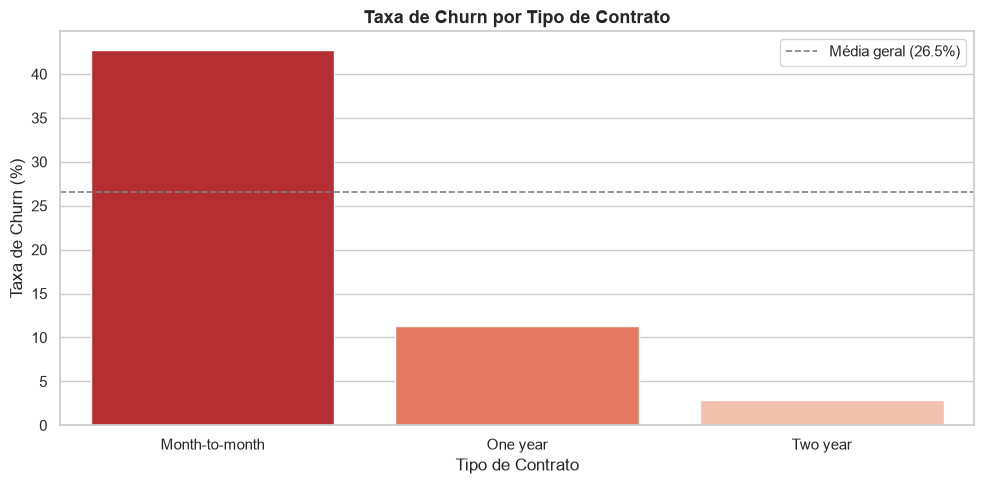
\includegraphics[width=.72\textwidth]{figuras/eda_contrato.png}
\caption{Taxa de cancelamento por tipo de contrato, com a média global (26,5\%) indicada pela linha tracejada.}
\label{fig:contrato}
\end{figure}

No plano financeiro, os clientes que cancelaram apresentam fatura mensal média
superior (R\$ 74,44 contra R\$ 61,27) e fatura acumulada média inferior
(R\$ 1.531,80 contra R\$ 2.549,91), diferença explicada pelo tempo de
relacionamento: 18,0 meses em média entre os que cancelaram e 37,6 meses entre
os que permaneceram. Todas as três diferenças são estatisticamente
significativas pelo teste de Mann-Whitney ($p < 0{,}001$). A distribuição do
tempo de relacionamento (Figura \ref{fig:tenure}) mostra concentração acentuada
de cancelamentos nos primeiros meses de contrato, padrão que motivou a criação
das faixas discretizadas e do indicador de cliente novo. A correlação de
Spearman com a variável alvo confirma o quadro: $\rho = -0{,}367$ para tempo de
relacionamento, $\rho = -0{,}230$ para fatura acumulada e $\rho = +0{,}185$ para
fatura mensal.

\begin{figure}[ht]
\centering
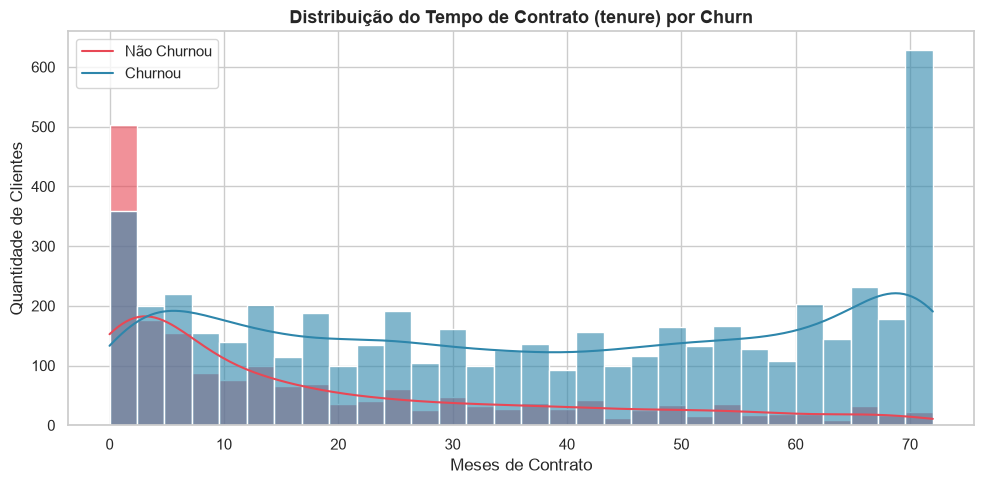
\includegraphics[width=.72\textwidth]{figuras/eda_tenure.png}
\caption{Distribuição do tempo de relacionamento (em meses) por situação de cancelamento.}
\label{fig:tenure}
\end{figure}

O escore de risco construído na etapa de engenharia de atributos
(Seção \ref{sub:features}) mostrou-se fortemente monotônico em relação à taxa de
cancelamento, o que valida a combinação de indicadores escolhida. Como mostra a
Tabela \ref{tab:score}, a taxa varia de 2,8\% no escore zero a 67,4\% no escore
máximo, uma razão de aproximadamente 24 vezes entre os extremos.

\begin{table}[ht]
\centering
\caption{Taxa de cancelamento por valor do escore de risco estendido.}
\label{tab:score}
\small
\begin{tabular}{|c|c|c|}
\hline
\textbf{Escore de risco} & \textbf{Clientes} & \textbf{Taxa de churn (\%)} \\
\hline
0 & 502   & 2,8  \\ \hline
1 & 720   & 7,8  \\ \hline
2 & 1.781 & 8,1  \\ \hline
3 & 1.579 & 22,5 \\ \hline
4 & 1.167 & 43,4 \\ \hline
5 & 950   & 58,9 \\ \hline
6 & 344   & 67,4 \\
\hline
\end{tabular}
\end{table}

\subsection{Seleção do modelo de churn}

Após 40 tentativas de otimização por algoritmo, os escores compostos obtidos em
validação cruzada foram muito próximos: 0,7031 para o XGBoost, 0,7014 para o
LightGBM e 0,6996 para o Random Forest. A Tabela \ref{tab:modelos} detalha as
métricas em validação cruzada de cinco dobras, cada modelo com o limiar
calibrado por sua própria varredura.

\begin{table}[ht]
\centering
\caption{Comparação dos modelos otimizados em validação cruzada de cinco dobras (conjunto de treino, 5.634 amostras). AUC = AUC-ROC; AP = \textit{average precision}; $S_{0{,}5}$ = escore composto da Equação \ref{eq:score}.}
\label{tab:modelos}
\small
\begin{tabular}{|l|c|c|c|c|c|c|c|}
\hline
\textbf{Modelo} & \textbf{AUC} & \textbf{AP} & \textbf{Acur.} & \textbf{Prec.} & \textbf{Rec.} & \textbf{F1} & \textbf{$S_{0{,}5}$} \\
\hline
XGBoost      & 0,847 & 0,659 & 0,806 & 0,663 & 0,542 & 0,597 & 0,703 \\ \hline
LightGBM     & 0,848 & 0,660 & 0,805 & 0,652 & 0,565 & 0,605 & 0,701 \\ \hline
Random Forest & 0,847 & 0,660 & 0,804 & 0,647 & 0,571 & 0,607 & 0,700 \\
\hline
\end{tabular}
\end{table}

A proximidade dos resultados é consistente com o achado de \cite{verbeke2012}
de que um grande grupo de classificadores tende a produzir desempenho comparável
em predição de churn, o que sugere que o fator limitante nesta base é o poder
informativo dos atributos disponíveis, e não a capacidade do algoritmo. O
XGBoost foi selecionado por apresentar o maior escore composto, com limiar
calibrado em 0,795. O valor elevado do limiar é consequência direta do fator
\textit{scale\_pos\_weight} aplicado durante o treinamento, que desloca as
probabilidades estimadas para cima; a calibração posterior reposiciona o ponto
de corte, e é por isso que reportar métricas com o limiar padrão de 0,5 seria
enganoso neste caso.

\subsection{Desempenho no conjunto de teste}

A Tabela \ref{tab:teste} apresenta as métricas do XGBoost no conjunto de teste
de 1.409 amostras, nunca utilizado durante treinamento, otimização ou
calibração. A Figura \ref{fig:avaliacao} mostra a matriz de confusão, a curva
ROC e a fronteira entre F1 e acurácia em função do limiar.

\begin{table}[ht]
\centering
\caption{Métricas do modelo XGBoost no conjunto de teste (\textit{hold-out}, 1.409 amostras, limiar 0,795).}
\label{tab:teste}
\small
\begin{tabular}{|l|c|l|c|}
\hline
\textbf{Métrica} & \textbf{Valor} & \textbf{Métrica} & \textbf{Valor} \\
\hline
AUC-ROC              & 0,847 & Precisão (churn) & 0,664 \\ \hline
\textit{Average precision} & 0,662 & \textit{Recall} (churn) & 0,540 \\ \hline
Acurácia             & 0,806 & F1 (churn)       & 0,596 \\
\hline
\end{tabular}
\end{table}

\begin{figure}[ht]
\centering
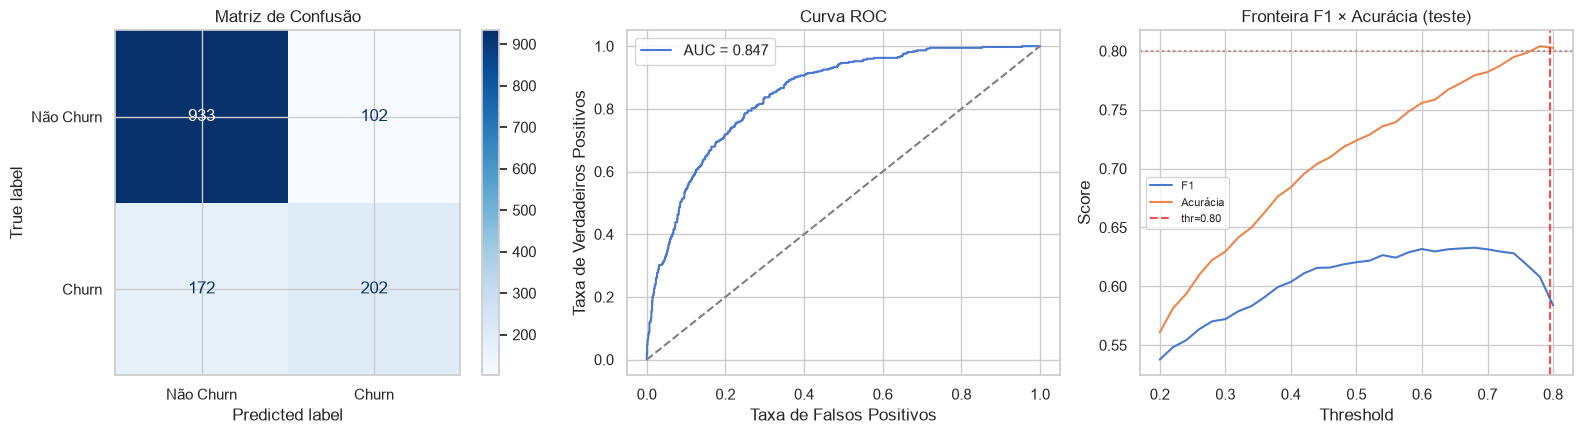
\includegraphics[width=\textwidth]{figuras/avaliacao_modelo.png}
\caption{Avaliação no conjunto de teste: matriz de confusão, curva ROC e fronteira entre F1 e acurácia por limiar de decisão.}
\label{fig:avaliacao}
\end{figure}

Em termos operacionais, das 374 ocorrências reais de cancelamento no conjunto de
teste, o modelo identificou 202 (verdadeiros positivos), deixou de identificar
172 (falsos negativos) e sinalizou incorretamente 102 clientes que não
cancelaram (falsos positivos). A leitura de negócio é direta: aproximadamente
dois de cada três clientes contatados por indicação do modelo cancelariam de
fato o serviço, contra uma taxa base de 26,5\% em uma abordagem sem modelo, o
que representa um ganho de precisão de cerca de 2,5 vezes sobre a seleção
aleatória.

As metas iniciais do projeto eram F1 e acurácia de 80\%. A meta de acurácia foi
atingida (80,6\%), mas a de F1 não (59,6\%). O painel direito da
Figura \ref{fig:avaliacao} evidencia por que se trata de um teto da base e não
de um problema de calibração: varrendo todo o intervalo de limiares, o F1 máximo
alcançável é de 63,7\% (em limiar 0,725) e a acurácia máxima é de 80,6\% (em
limiar 0,795, ou seja, exatamente o limiar calibrado). Não existe, portanto,
limiar capaz de satisfazer simultaneamente as duas metas com os atributos
disponíveis, e a calibração já opera no ponto de acurácia máxima. Esse é
um resultado relevante do estudo piloto: a base IBM Telco não possui atributos
comportamentais de consumo, de atendimento ou de qualidade de serviço, que são
justamente os que elevam o desempenho em trabalhos com dados reais de
operadoras, como o AUC de 93,3\% obtido por \cite{ahmad2019} com atributos de
rede social.

\subsection{Interpretabilidade: o que o modelo está usando}
\label{sub:res-shap}

A Figura \ref{fig:shapglobal} apresenta a distribuição dos valores SHAP das 15
variáveis mais influentes no conjunto de teste, ordenadas pela média do valor
absoluto das contribuições. O resultado mais relevante é que as duas variáveis
no topo do \textit{ranking} são derivadas, e não colunas originais da base: a
interação entre fatura mensal e contrato mensal
($\overline{|\phi|} = 0{,}636$) e o escore de risco estendido
($0{,}432$), ambas construídas na etapa de engenharia de atributos a partir dos
achados exploratórios. A terceira posição é do tempo de relacionamento
($0{,}322$), seguida pelo indicador de contrato de dois anos ($0{,}180$), pela
fatura média por mês de permanência ($0{,}143$) e pela fatura acumulada
($0{,}140$). A interação entre tempo curto de relacionamento e fibra óptica
aparece em nono lugar ($0{,}110$).

\begin{figure}[ht]
\centering
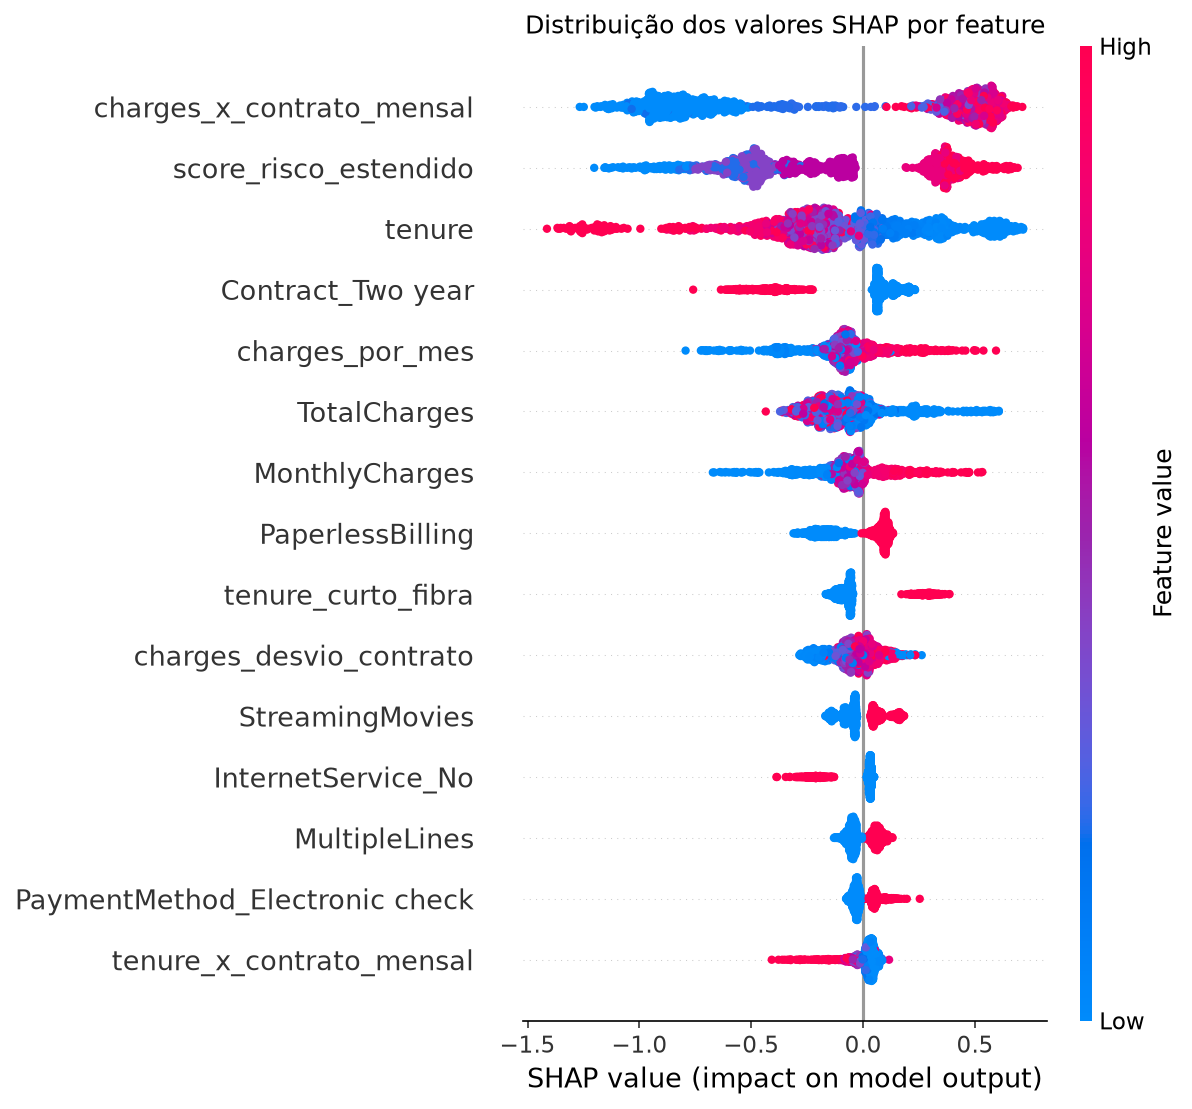
\includegraphics[width=.82\textwidth]{figuras/shap_beeswarm.png}
\caption{Valores SHAP das 15 variáveis mais influentes no conjunto de teste. Cada ponto é um cliente; a cor indica o valor do atributo (azul baixo, vermelho alto) e a posição horizontal indica a contribuição para a predição.}
\label{fig:shapglobal}
\end{figure}

Além da ordenação, o sentido dos efeitos confirma a coerência entre o modelo e a
análise exploratória. No tempo de relacionamento, os pontos vermelhos (valores
altos) concentram-se à esquerda, com contribuição negativa, ou seja, mais tempo
de casa reduz o risco estimado --- exatamente o sinal da correlação de Spearman
de $-0{,}367$ observada na Seção \ref{sub:res-eda}. O indicador de contrato de dois anos, quando
ativo, produz contribuição fortemente negativa, consistente com a taxa de
cancelamento de apenas 2,8\% naquele grupo. Já a interação de tempo curto com
fibra óptica contribui positivamente quando ativa, o que antecipa o perfil do
segmento 2 identificado na etapa de agrupamento.

Esse quadro sustenta duas conclusões. A primeira é que a engenharia de atributos
foi determinante: as variáveis construídas dominam a predição, e sua importância
não decorre de artefato estatístico, pois o sentido dos efeitos reproduz relações
já verificadas de forma independente na exploração. A segunda é que o modelo não
está apoiado em variáveis demográficas --- gênero, por exemplo, não aparece entre
as 15 primeiras ---, mas em comportamento contratual e financeiro, o que é
desejável tanto do ponto de vista de negócio quanto do ponto de vista de
equidade da decisão automatizada.

\begin{figure}[ht]
\centering
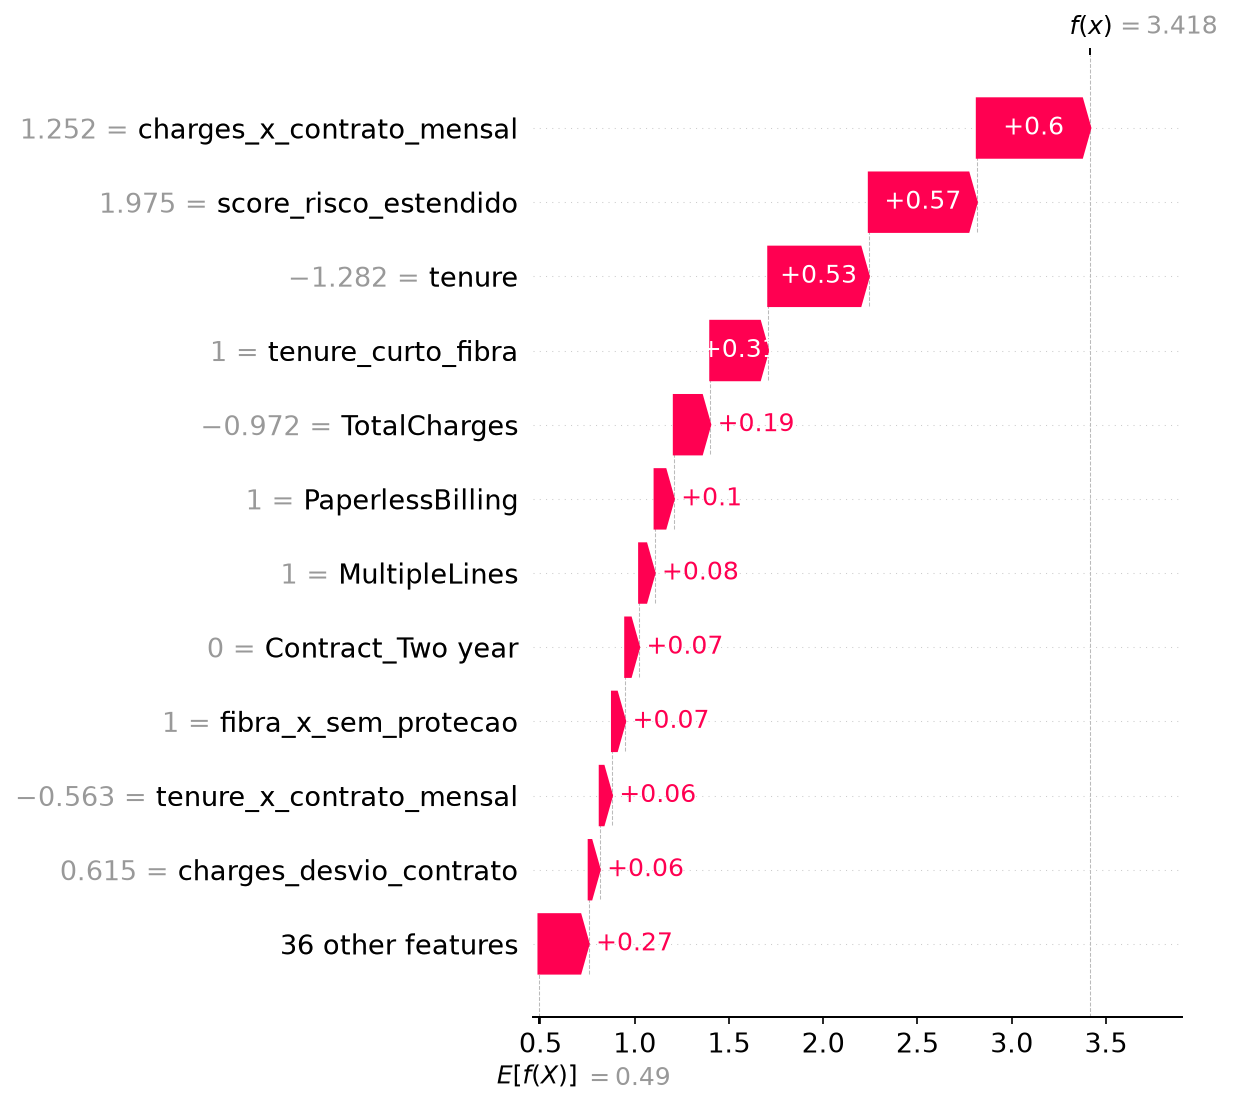
\includegraphics[width=.78\textwidth]{figuras/shap_waterfall.png}
\caption{Decomposição individual da predição do cliente de maior probabilidade estimada no conjunto de teste, do valor esperado do modelo ($E[f(X)] = 0{,}49$) até a predição final ($f(x) = 3{,}418$), em escala de \textit{log-odds}.}
\label{fig:shapwater}
\end{figure}

A Figura \ref{fig:shapwater} exemplifica a leitura local com o cliente de maior
probabilidade estimada no teste (0,968, com cancelamento efetivamente
confirmado). A predição parte do valor esperado do modelo, $0{,}49$ em
\textit{log-odds}, e chega a $3{,}418$ pela soma de contribuições positivas, com
destaque para a interação fatura-contrato mensal ($+0{,}60$), o escore de risco
estendido ($+0{,}57$), o tempo de relacionamento curto ($+0{,}53$) e a
combinação de tempo curto com fibra ($+0{,}30$). É esse tipo de decomposição que
viabiliza a personalização da abordagem: para este cliente, a explicação indica
que a ação deveria atacar simultaneamente o vínculo contratual e o valor da
fatura, e não, por exemplo, o portfólio de serviços agregados.

\subsection{Escoragem e população em risco}

Aplicado à base completa com o limiar de 0,795, o modelo sinalizou 1.556
clientes como em risco, o que corresponde a 22,1\% da base. Entre esses
clientes, a taxa real de cancelamento é de 69,5\%, contra 26,5\% na base
completa, e a probabilidade média estimada é de 0,881. É importante registrar a
natureza desse número: como 80\% da base foi utilizada no treinamento, a taxa de
69,5\% entre os sinalizados é otimista por conter registros vistos pelo modelo.
A estimativa não enviesada de precisão é a do conjunto de teste, 66,4\%. A
escoragem completa é usada aqui como insumo operacional para a segmentação, não
como medida de desempenho.

\subsection{Segmentação dos clientes em risco}

A varredura de K de 2 a 10 sobre os 1.556 clientes sinalizados indicou K = 3
como valor de maior coeficiente de silhueta, com 0,283, coincidindo com o valor
adotado por critério de negócio --- três perfis são mais acionáveis para uma
equipe comercial que uma divisão binária genérica. A Figura \ref{fig:selecaok}
apresenta a inércia e a silhueta em função de K.

\begin{figure}[ht]
\centering
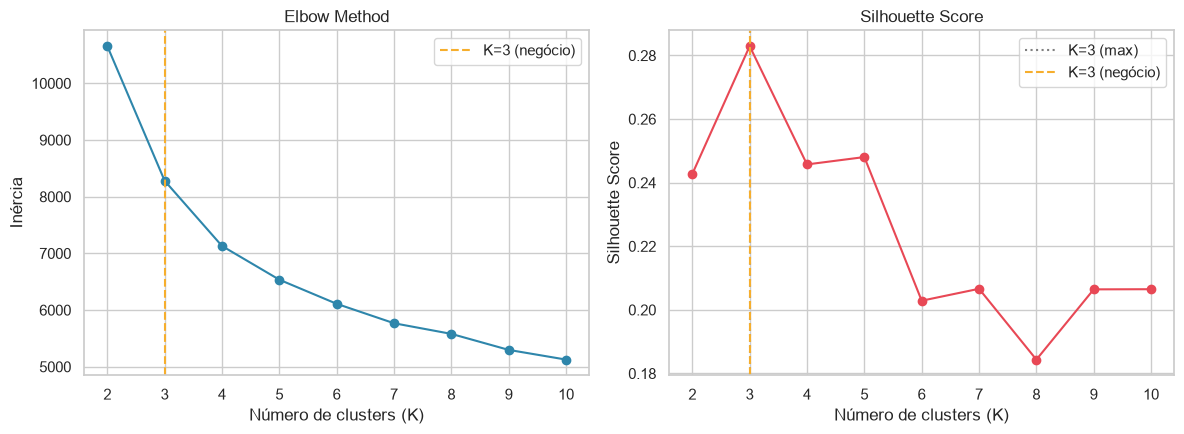
\includegraphics[width=\textwidth]{figuras/selecao_k.png}
\caption{Escolha do número de grupos: método do cotovelo (esquerda) e coeficiente de silhueta (direita).}
\label{fig:selecaok}
\end{figure}

O valor absoluto da silhueta, 0,283, indica grupos com sobreposição
considerável. Isso é esperado neste cenário: a população segmentada já é
homogênea por construção, pois todos os seus membros foram selecionados pelo
mesmo critério de alto risco, o que reduz a separação natural entre subgrupos.
A projeção bidimensional por componentes principais (Figura \ref{fig:pca}),
que retém 51,5\% da variância, mostra grupos visualmente distinguíveis, porém
com fronteiras contíguas.

\begin{figure}[ht]
\centering
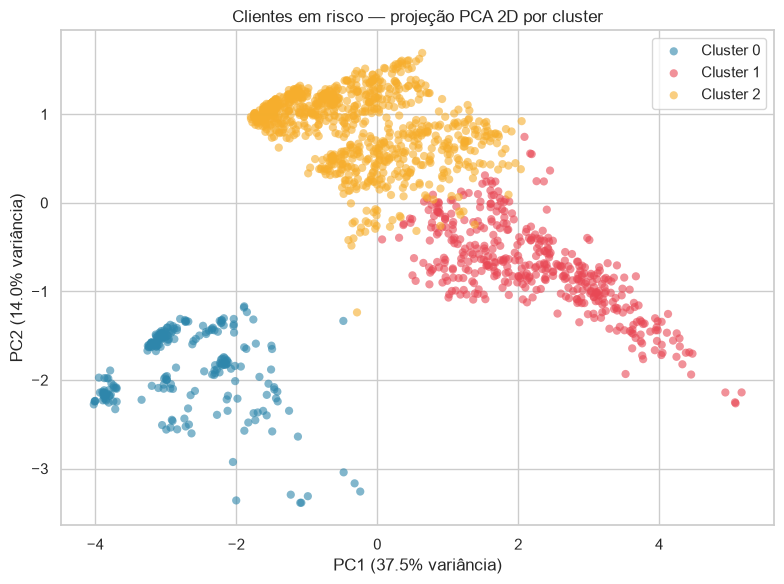
\includegraphics[width=.68\textwidth]{figuras/pca_clusters.png}
\caption{Projeção em duas componentes principais dos 1.556 clientes em risco, coloridos por grupo.}
\label{fig:pca}
\end{figure}

O DBSCAN, executado sobre dez componentes principais com raio de vizinhança
igual a 3,0 e mínimo de dez amostras, convergiu para um único grupo, sem
classificar nenhum ponto como ruído. O comportamento reforça a leitura anterior:
não há regiões de baixa densidade separando subpopulações nesse espaço, de modo
que um método baseado em densidade não encontra estrutura útil. O K-Means foi
mantido por produzir grupos mutuamente exclusivos, sem clientes órfãos, o que é
um requisito prático para a operacionalização de campanhas.

A Tabela \ref{tab:perfis} caracteriza os três segmentos e a
Figura \ref{fig:perfil} mostra o mesmo perfil em forma de mapa de calor. Os
grupos separam-se com clareza em duas dimensões interpretáveis: o tempo de
relacionamento e o patamar de fatura combinado ao tipo de acesso.

\begin{table}[ht]
\centering
\caption{Perfil médio dos três segmentos de clientes em risco.}
\label{tab:perfis}
\small
\begin{tabular}{|l|c|c|c|}
\hline
\textbf{Característica} & \textbf{Segmento 0} & \textbf{Segmento 1} & \textbf{Segmento 2} \\
\hline
Clientes                        & 241 & 427 & 888 \\ \hline
Participação nos sinalizados (\%) & 15,5 & 27,4 & 57,1 \\ \hline
Tempo de relacionamento (meses) & 2,7 & 26,7 & 4,8 \\ \hline
Fatura mensal média (R\$)       & 42,47 & 94,54 & 81,93 \\ \hline
Internet predominante           & DSL & Fibra & Fibra \\ \hline
Fibra sem suporte técnico (\%)  & 0,0 & 85,9 & 91,8 \\ \hline
Sem serviços de proteção (\%)   & 73,0 & 37,9 & 62,8 \\ \hline
Probabilidade média estimada    & 0,850 & 0,848 & 0,905 \\ \hline
Taxa real de cancelamento (\%)  & 65,6 & 66,5 & 72,1 \\
\hline
\end{tabular}
\end{table}

\begin{figure}[ht]
\centering
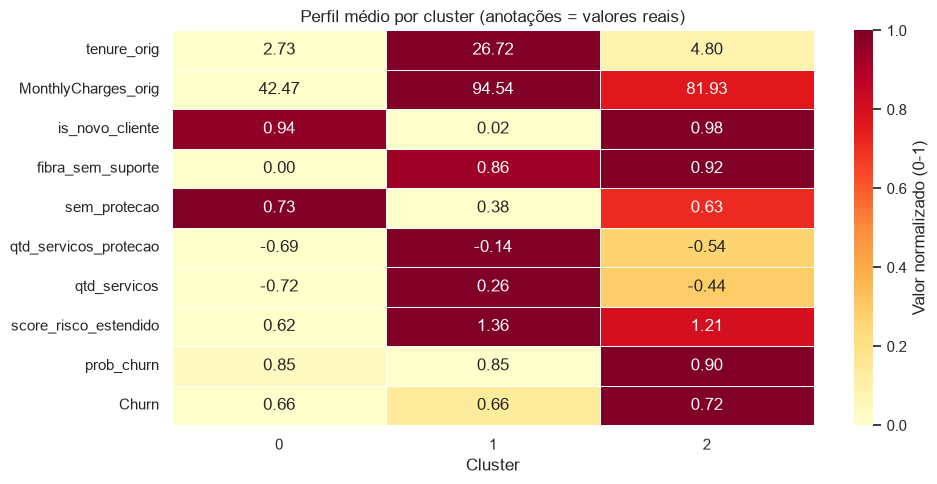
\includegraphics[width=.92\textwidth]{figuras/perfil_clusters.png}
\caption{Mapa de calor do perfil médio por segmento; a cor indica o valor normalizado e as anotações os valores reais.}
\label{fig:perfil}
\end{figure}

O segmento 0 reúne clientes muito recentes (2,7 meses em média), com acesso DSL
e fatura baixa (R\$ 42,47), em geral sem serviços de proteção contratados. O
segmento 1 é o oposto no eixo temporal: clientes com relacionamento longo (26,7
meses), fibra óptica e a maior fatura média (R\$ 94,54), sendo que 85,9\% não
possuem suporte técnico contratado. O segmento 2 concentra a maioria dos
sinalizados (57,1\%) e combina os fatores de maior risco: relacionamento curto
(4,8 meses), fibra óptica sem suporte técnico em 91,8\% dos casos e fatura
média-alta (R\$ 81,93). Coerentemente, é o segmento com maior probabilidade
média estimada (0,905) e maior taxa real de cancelamento (72,1\%).

\subsection{Impacto financeiro e plano de retenção}

A soma das faturas mensais dos 1.556 clientes sinalizados totaliza
R\$ 123.361,85, o que corresponde a uma exposição anual projetada de
R\$ 1.480.342,20 caso nenhuma ação de retenção seja tomada. A distribuição
dessa exposição entre os segmentos é bastante desigual, como mostram a
Tabela \ref{tab:impacto} e a Figura \ref{fig:impacto}.

\begin{table}[ht]
\centering
\caption{Receita exposta por segmento.}
\label{tab:impacto}
\small
\begin{tabular}{|c|c|c|c|c|}
\hline
\textbf{Segmento} & \textbf{Clientes} & \textbf{Receita mensal (R\$)} & \textbf{Part. (\%)} & \textbf{Projeção anual (R\$)} \\
\hline
0 & 241 & 10.235,55 & 8,3  & 122.826,60 \\ \hline
1 & 427 & 40.369,85 & 32,7 & 484.438,20 \\ \hline
2 & 888 & 72.756,45 & 59,0 & 873.077,40 \\ \hline
\textbf{Total} & \textbf{1.556} & \textbf{123.361,85} & \textbf{100,0} & \textbf{1.480.342,20} \\
\hline
\end{tabular}
\end{table}

\begin{figure}[ht]
\centering
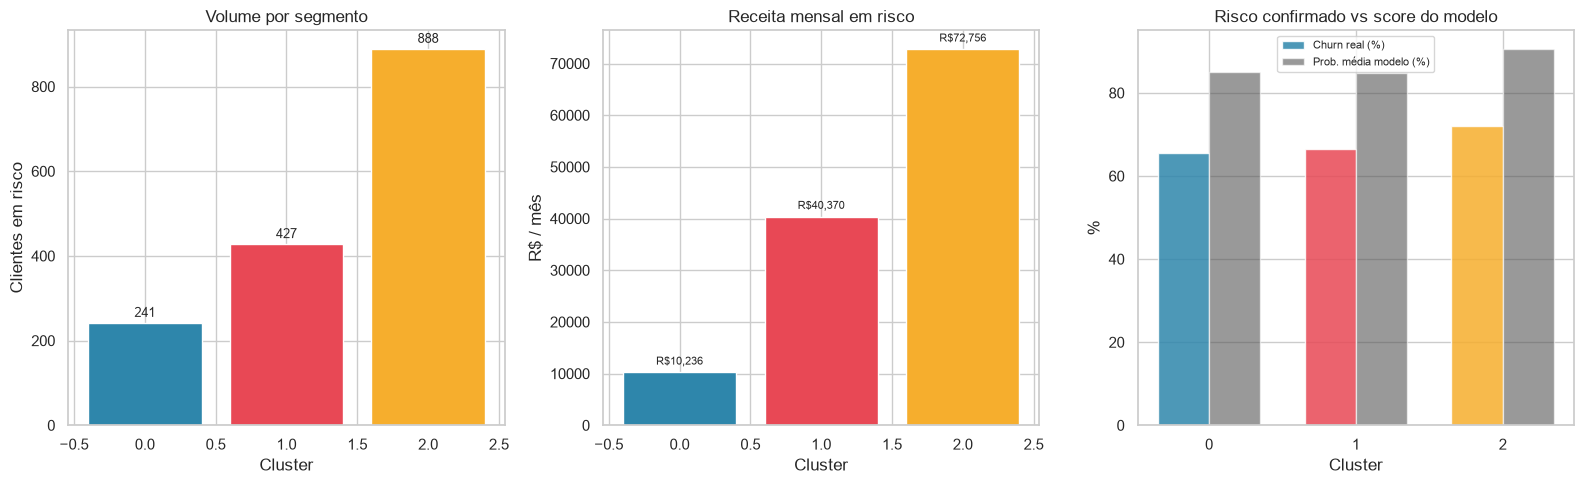
\includegraphics[width=\textwidth]{figuras/impacto_clusters.png}
\caption{Impacto por segmento: volume de clientes, receita mensal exposta e comparação entre cancelamento real e probabilidade média estimada.}
\label{fig:impacto}
\end{figure}

O contraste entre volume e valor é o principal resultado gerencial da
segmentação. O segmento 0 representa 15,5\% dos clientes sinalizados, mas apenas
8,3\% da receita exposta; o segmento 1 representa 27,4\% dos clientes e 32,7\%
da receita; e o segmento 2 concentra 57,1\% dos clientes e 59,0\% da receita
exposta. Uma abordagem única para toda a lista de 1.556 clientes trataria da
mesma forma casos com fatura média de R\$ 42,47 e de R\$ 94,54, o que é
economicamente ineficiente: o custo de um contato humano se justifica no segundo
caso e não no primeiro.

Com base nesses perfis foi elaborado o plano de retenção resumido na
Tabela \ref{tab:playbook}. A lógica de diferenciação combina o valor exposto,
que define o custo aceitável do canal de contato, e a causa provável do risco,
que define a oferta. Para o segmento 0, de baixo valor e relacionamento muito
recente, a hipótese é de atrito de adoção, endereçada por integração assistida
em canais automatizados de baixo custo. Para o segmento 1, de alto valor e
relacionamento longo, a hipótese é de insatisfação silenciosa associada à
ausência de suporte técnico, endereçada por contato consultivo humano com oferta
de pacote de suporte. Para o segmento 2, o mais crítico em risco e em valor
agregado, a hipótese combina relacionamento recente e possível problema de
qualidade de acesso em fibra, endereçada por contato imediato com diagnóstico
técnico e desconto condicionado à migração para contrato anual --- justamente o
tipo de contrato que a análise exploratória apontou como o de menor taxa de
cancelamento.

\begin{table}[ht]
\centering
\caption{Plano de retenção diferenciado por segmento.}
\label{tab:playbook}
\small
\begin{tabular}{|c|l|c|l|}
\hline
\textbf{Seg.} & \textbf{Perfil} & \textbf{Prior.} & \textbf{Ação e indicador de acompanhamento} \\
\hline
0 & Novos DSL,      & Média   & Integração proativa em D+7 e D+30 por canais \\
  & fatura baixa    &         & automatizados; oferta de plano anual com 10\% \\
  &                 &         & de desconto. KPI: conversão para contrato \\
  &                 &         & anual em 60 dias. \\ \hline
1 & Veteranos fibra,& Alta    & Contato consultivo humano em até 48h; pacote \\
  & fatura alta     &         & de suporte técnico e segurança gratuito por \\
  &                 &         & 3 meses. KPI: retenção em 90 dias e adesão \\
  &                 &         & ao pacote de suporte. \\ \hline
2 & Novos fibra,    & Crítica & Contato imediato em 24h com diagnóstico de \\
  & maior risco     &         & qualidade de sinal; desconto de 15\% por 6 \\
  &                 &         & meses condicionado a contrato anual. KPI: \\
  &                 &         & redução de cancelamento em 30 dias. \\
\hline
\end{tabular}
\end{table}

\subsection{Limitações}
\label{sub:limitacoes}

O estudo apresenta limitações que delimitam a interpretação dos resultados.
A primeira é o teto de desempenho da base: a meta de F1 de 80\% não foi
atingida e a evidência da Figura \ref{fig:avaliacao} indica que ela não é
alcançável com os atributos disponíveis, uma vez que a base não contém dados de
consumo, de histórico de atendimento ou de qualidade de serviço. A segunda é a
ausência de dimensão temporal, que impede validação com separação por período e
impossibilita o uso de modelos de sobrevivência, mais adequados para estimar
\textit{quando} o cancelamento ocorreria e não apenas \textit{se} ocorreria.

A terceira limitação é a qualidade moderada da estrutura de agrupamento: a
silhueta de 0,283 e o resultado do DBSCAN indicam que os segmentos são cortes
úteis de uma população contínua, e não grupos naturalmente separados. A quarta é
a natureza da métrica financeira: a receita exposta é uma medida de exposição
bruta, e não de perda esperada, pois não incorpora a probabilidade individual de
cancelamento, o custo da campanha nem a taxa de sucesso da intervenção. A quinta
é que a validação do plano de retenção exigiria experimentação em produção, com
grupo de controle, o que está fora do escopo de um estudo piloto sobre base
pública. Por fim, os valores SHAP explicam o \textbf{modelo}, e não o fenômeno:
eles indicam em que atributos a predição se apoia, mas não estabelecem relação
causal. Afirmar que reduzir a fatura de um cliente reduziria seu risco de
cancelamento exigiria evidência experimental, não apenas a contribuição SHAP
positiva desse atributo. A análise também se restringiu ao conjunto de teste,
que é a leitura correta para avaliação, mas não cobre a base completa escorada.

\section{Conclusão}
\label{sec:5}

Este trabalho desenvolveu um \textit{pipeline} de duas etapas para predição e
qualificação de risco de cancelamento em telecomunicações, sobre a base pública
IBM Telco Customer Churn. A etapa de classificação comparou três algoritmos de
conjunto otimizados por busca bayesiana com objetivo composto entre F-medida e
acurácia, selecionando o XGBoost com AUC-ROC de 0,847, acurácia de 80,6\% e
precisão de 66,4\% no conjunto de teste. A análise SHAP mostrou que as duas
variáveis mais influentes são derivadas --- a interação entre fatura mensal e
contrato mensal e o escore de risco estendido ---, com sentidos de efeito
coerentes com a exploração. A etapa de segmentação aplicou K-Means com K = 3
exclusivamente sobre os 1.556 clientes sinalizados como em risco, produzindo
três perfis interpretáveis que foram quantificados em R\$ 123,4 mil de receita
mensal exposta, com 59,0\% concentrados em um único segmento.

Quatro conclusões se destacam. Primeiro, o encadeamento entre classificação e
segmentação agrega valor real de decisão: a mesma lista de clientes em risco,
quando desdobrada por perfil, revela que volume e valor não caminham juntos, o
que permite alocar canais de contato de custos distintos de forma
economicamente justificada. Segundo, a calibração explícita do limiar de decisão
como parte do objetivo de otimização é mais relevante que a escolha do algoritmo
neste problema, já que os três modelos avaliados apresentaram desempenho
praticamente equivalente, o que é consistente com os \textit{benchmarks} da
literatura \cite{verbeke2012}. Terceiro, a engenharia de atributos foi o
principal fator de ganho, e a análise SHAP permitiu verificar isso de forma
objetiva: as variáveis derivadas lideram a importância e reproduzem, no sentido
dos efeitos, as relações identificadas na exploração. Quarto, o diagnóstico do
teto de desempenho é, em si, um resultado útil do estudo piloto: ele indica que
ganhos adicionais dependem de enriquecimento da base, e não de refinamento
adicional do modelo.

Como trabalhos futuros, destacam-se cinco direções. A primeira é o
enriquecimento da base com atributos comportamentais e de qualidade de serviço
--- volume de tráfego, chamados de suporte, indicadores de estabilidade da
conexão --- que a literatura aponta como determinantes para superar o patamar de
desempenho observado \cite{ahmad2019}. A segunda é a substituição da métrica de
exposição bruta por um modelo de perda esperada e de retorno da campanha,
incorporando probabilidade individual, custo de contato e taxa de conversão, na
linha da avaliação orientada a lucro proposta por \cite{verbeke2012}. A terceira
é a incorporação de dimensão temporal para permitir análise de sobrevivência e
validação por período. A quarta é o uso operacional das explicações individuais
já produzidas, associando cada motivo dominante de risco a uma oferta específica,
de modo a personalizar a abordagem em nível de cliente e não apenas por
segmento. A quinta é a validação experimental do plano de retenção por meio de
teste controlado, comparando os segmentos tratados com um grupo de controle, o
que permitiria também avançar para modelagem de \textit{uplift}, em que o alvo
passa a ser o efeito incremental da ação e não a probabilidade de cancelamento.

\section{Links}

\begin{itemize}
    \item Link para o vídeo da apresentação: http://

    \item Link para os dados do projeto piloto (códigos, bases de dados): http://

\end{itemize}

\bibliographystyle{sbc}
\bibliography{referencias}

\end{document}
